\titledquestion{Mix av vektorer}

Med hjälp av olika kombinationer av två givna vektorer kan man skapa alla andra vektorer, förutsatt att de två givna vektorerna inte är parallella.

\begin{figure}[H]
    \centering
    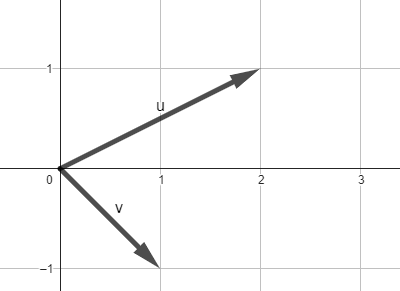
\includegraphics[width=0.5\linewidth]{img/vektorer.png}
    \caption{De två givna vektorerna.}
\end{figure}

\begin{parts}
    \part Skriv upp $\vec{u}$ och $\vec{v}$ på koordinatform.
    \part Uttryck vektorn $\vec{w}=(0,3)$ med hjälp av $\vec{u}$ och $\vec{v}$. Lös uppgiften både grafiskt och algebraiskt. 
    \part Uttryck vektorn $\vec{t}=(11,10)$ med hjälp av $\vec{u}$ och $\vec{v}$. 
    \begin{rem}
        Vi har nyss lärt oss ekvationssystem...
    \end{rem}
\end{parts}